\documentclass[14pt]{extarticle}
\usepackage{fontspec}
\usepackage[ukrainian]{babel}
\usepackage[contents=TODO, color=gray, pages=some]{background}
\usepackage[a4paper, left=20mm, top=20mm, right=10mm, bottom=20mm]{geometry}
\usepackage{indentfirst}
\usepackage{titlesec}
\usepackage{stringstrings}
\usepackage{fancyhdr}
\usepackage{enumitem}
\usepackage{tabularx}
\usepackage[hidelinks]{hyperref}
\usepackage{textcase}
\usepackage{url}
\usepackage{csquotes}
\usepackage[style=numeric, sorting=none]{biblatex}
\usepackage{graphicx}
\usepackage{float}
\usepackage{caption}
\usepackage{listings}
\usepackage{rotating}

\lstnewenvironment{mycode}[1][]{
  \lstset{
    basicstyle=\small\ttfamily,
    captionpos=b,
    #1
  }
}{}

\DeclareCaptionLabelFormat{dstuFigLabel}{Рисунок #2}
\DeclareCaptionLabelSeparator{abobasep}{ --- }
\captionsetup[figure]{labelformat = dstuFigLabel
                     ,labelsep    = abobasep
                     }

\addbibresource{zapiska.bib}

% TODO: make section uppercase in embedded links

% Uppercase sections in ToC
\makeatletter
\let\oldcontentsline\contentsline
\def\contentsline#1#2{%
  \expandafter\ifx\csname l@#1\endcsname\l@section
    \expandafter\@firstoftwo
  \else
    \expandafter\@secondoftwo
  \fi
  {%
    \oldcontentsline{#1}{\MakeTextUppercase{#2}}%
  }{%
    \oldcontentsline{#1}{#2}%
  }%
}
\makeatother

\hypersetup{linktoc=all}

\pagestyle{fancy}
\fancyhf{}
\fancyhead[R]{\thepage}
\renewcommand{\headrule}{}
\setlength{\headheight}{17pt}

\setmainfont{Times New Roman}
\linespread{1.5}
\setlength{\parindent}{16mm}

\titleformat{\section}
  { \filcenter % center
    \fontsize{14pt}{14pt}
    \bfseries % semi bold
    \MakeUppercase
  }
  {\thesection~}
  {0pt}
  {}
\titlespacing*{\section}{0pt}{12pt}{6pt}

\titleformat{\subsection}
  { \fontsize{14pt}{14pt}
  }
  % TODO: sentence case
  {\thesubsection~}
  {0pt}
  {}
\titlespacing*{\subsection}{0pt}{6pt}{0pt}

\titleformat{\subsubsection}
  { \fontsize{14pt}{14pt}
  }
  % TODO: sentence case
  {\thesubsubsection~}
  {0pt}
  {}
\titlespacing*{\subsubsection}{0pt}{6pt}{0pt}

% all sections will start at new page
\let\oldsection\section
\renewcommand{\section}{\clearpage\oldsection}

\newcommand{\unnumberedSection}[1]{%
  \section*{#1}%
  \phantomsection
  \addcontentsline{toc}{section}{#1}%
}

\newcommand{\unnumberedSubsection}[1]{%
  \subsection*{#1}%
  \addcontentsline{toc}{subsection}{#1}%
}

\begin{document}


титульний аркуш
\BgThispage
\thispagestyle{empty}

\newpage
завдання
\BgThispage
\section*{реферат}
\BgThispage

% зміст
\tableofcontents

\unnumberedSection{ПЕРЕЛІК УМОВНИХ ПОЗНАК, СИМВОЛІВ, СКОРОЧЕНЬ І ТЕРМІНІВ}
УДК --- Універсальна десяткова класифікація

НР --- наукова робота

% ommited because it's only used for groupping
% основну частину:
  \unnumberedSection{ВСТУП}  
  Задача, яку розглядає дана робота ---
  переклад та перевірка точності перекладу текстів \cite{wiki_nlp} (НР)
  з природної мови на формальну (шифр УДК).
  
  Точність УДК шифрів є ключовою для ефективної класифікації
  та пошуку наукової літератури.
  Однак, ручний вибір та перевірка УДК шифрів вимагає значних зусиль,
  займає багато часу та супроводжується високим ризиком виникнення помилок.
  Зовнішня перевірка може зменшити ризик помилок, але вимагає додаткових зусиль.
  Натомість, автоматизоване рішення може значно зменшити час та ресурси,
  необхідні для вибору та перевірки, а також мінімізувати ризик помилок.
  Тому ця робота має на меті розробити надійний
  та ефективний автоматизований інструмент для вибору
  та перевірки УДК шифрів НР.

  % ommited because it's only used for groupping
  % основний текст кваліфікаційного проєкту (роботи):

  \section{ЗБІР ТА АНАЛІЗ ВИМОГ}

  \subsection{Універсальна десяткова класифікація}
  Універсальна десяткова класифікація (УДК) \cite{udc_wiki} —--
  бібліографічна та бібліотечна класифікація,
  представляє систематичне впорядкування всіх галузей людських знань,
  організованих як узгоджена система,
  у якій галузі знань заємопов’язані.
  
  В УДК використовуються арабські цифри в десятковому порядку.
  Кожне число розглядається як десятковий дріб
  з опущеною початковою десятковою крапкою, яка визначає порядок запису.
  Для зручності читання УДК зазвичай ставиться розділовий знак
  після кожної третьої цифри.

  Основні таблиці \cite{udc_structure_and_tables} містять різні дисципліни та галузі знань,
  розташовані в 9 основних класах, пронумерованих від 0 до 9
  (при цьому 4 клас є вільним).
  На початку кожного класу також є серія спеціальних допоміжних слів,
  які виражають аспекти, що повторюються в цьому конкретному класі.
  Основні таблиці в УДК містять понад 60 000 підрозділів.
  \begin{enumerate}
      [labelindent=\dimexpr\parindent*2\relax, leftmargin=*, start=0]
    \item Наука і знання.
    Організація.
    Комп'ютерна наука.
    Інформатика.
    Документація.
    Бібліотечна справа.
    Заклади.
    Публікації
    \item Філософія. Психологія
    \item Релігія. Теологія
    \item Суспільствознавство
    \item -
    \item Математика. Природничі науки
    \item Прикладні науки. Медицина, Техніка
    \item Мистецтво. Розваги. Спорт
    \item Мовознавство. Література
    \item Географія. Історія
  \end{enumerate}

  Загальні допоміжні засоби — концепції,
  які можна використовувати в поєднанні
  з будь-яким іншим кодом УДК з основних класів
  або з іншими загальними допоміжними засобами.
  Вони мають унікальні позначення, що виділяють їх у складних виразах.
  Звичайні допоміжні числа завжди починаються з певного символу,
  напр. = (знак рівності) завжди вводить поняття,
  що представляють мову документа;
  (0...) цифри в круглих дужках, починаючи з нуля,
  завжди представляють поняття, що позначає форму документа.
  Таким чином (075) підручник і =111 англійська мова може бути об’єднана,
  щоб виразити, наприклад, (075)=111 підручники англійською мовою,
  і в поєднанні з числами з основних таблиць
  УДК їх можна використовувати таким чином:
  2(075)=111 підручники з релігії англійською мовою,
  51(075)=111 Підручники з математики англійською мовою та ін.

  \begin{tabularx}{\dimexpr\linewidth - \parindent\relax}{cX}
    =... & Загальні допоміжні засоби мови. \\
    (0...) & Загальні допоміжні форми форми. \\
    (1/9) & Загальні допоміжні слова місця. \\
    (=...) & Загальні допоміжні ознаки людського походження,
    етнічної групи та національності. \\
    "..." & Загальні допоміжні слова часу,
    допомагає зробити хвилинний поділ часу, наприклад: "1993-1996" \\
    -0... & Загальні допоміжні характеристики загальних характеристик:
    Властивості, Матеріали, Відносини/Процеси та Особи. \\
    -02 & Загальні допоміжні властивості. \\
    -03 & Загальні допоміжні матеріали. \\
    -04 & Загальні допоміжні елементи відносин, процесів і операцій. \\
    -05 & Загальні допоміжні особи та особисті характеристики. \\
  \end{tabularx}

  Доступно кілька сполучних символів для зв’язку та розширення номерів УДК:

  \begin{tabular}{|l|l|}
    \hline
    Символ & Значення \\
    + & узгодження, доповнення \\
    / & послідовне розширення \\
    : & відношення \\
    $[~~]$ & підгрупування \\
    $*$ & Впроваджує нотацію, відмінну від УДК \\
    A/Z & Пряма алфавітна специфікація \\
    \hline
  \end{tabular}

  \subsection{Аналіз проблеми}
  Мета роботи ---
  розробити ПЗ для підбору та перевірки коректності УДК шифрів НР.
  Під підбором розуміється наступний функціонал --- на вході маємо текст роботи,
  на виході --- список класів та підкласів УДК (далі --- класів),
  до яких ця робота належить.
  Перевірка --- на вході маємо текст роботи та шифр,
  на виході --- згенерований шифр та оцінку схожості наданого
  та згенерованого шифрів, яким саме чином ця оцінка буде отримана,
  та як вона буде виглядати розглянемо в наступних розділах.
  
  Програму можна узагальнити до такої специфікації ---
  на вході маємо текст роботи та опціонально шифр,
  на виході маємо список класів та, якщо був наданий шифр,
  порівняльну оцінку зі згенерованими класами.

  Через те що наукові роботи можуть бути доступні у різноманітних форматах,
  варто уточнити що ПЗ буде приймати їх
  у форматі plain-text на англійській мові.

  Це можна розглядати як проблему класифікації
  \cite{multiclass_classification_wiki, statistical_classification_wiki}
  --- маємо множину об'єктів,
  які певним чином розподілені на класи (підмножини).
  Задача класифікації ---
  різновид машинного навчання
  \cite{machine_learning_wiki} (англ. machine learning, далі —-- ML).
  Розрізняють два типи навчання:
  \begin{itemize}[labelindent=\dimexpr\parindent*2\relax, leftmargin=*]
    \item навчання з учителем (англ. supervised learning) ---
    комп'ютеру надається набір даних (data set),
    в якому даним вже надано бажаний результат ---
    саме за ним комп'ютер і буде навчатись.

    \item навчання без учителя (англ. unsupervised learning) ---
    набір даних, наданий комп'ютеру, ніяк не помічається ---
    комп'ютер сам має розбити дані на деякі групи (clustering).
  \end{itemize}

  Класи заздалегідь відомі, тож навчання без учителя, в нашому випадку,
  не підходить. Крім того можна використати існуючи класифіковані роботи,
  як набір даних для навчання.
  Але отримання достатнього набору даних вимагає великих зусиль ---
  потрібно отримати декілька робіт для кожного класу та підкласу
  та їх різних комбінацій. Тож пропонується простіший алгоритм:
  \begin{enumerate}[labelindent=\dimexpr\parindent*2\relax, leftmargin=*]
    \item Витягнемо з тексту роботи ключові слова. \cite{keyword_extraction_wiki}
    \item Порівняемо ключові слова із термінами та поняттями у каталозі УДК.
  \end{enumerate}

  Останній крок є дещо проблематичним
  через те що доступ до офіційного каталогу здійснюється на платній основі ---
  такий варіант не підходить для даного випадку через відсутність фінансування.
  Але існують безкоштовні та/або відкриті каталоги
  \cite{udc_summary, udc_summary_linked},
  які можна використати замість платної версії.
  Авжеж вони мають свої недоліки, наприклад: менша частота оновлень,
  менший корпус інформації, тощо.
  Не дивлячись на ці недоліки
  вони є достатнім ресурсом для початкової версії ПЗ.
  Також за бажанням ПЗ може бути відредагованим
  у майбутньому щоб використовувати платну версію.

  \subsection{Огляд аналогів}
  Широкодоступних аналогів, які б повністю відтворювали функціонал ---
  підбір кодів (або в нашому випадку класів) УДК та їх порівняння/перевірка,
  не знайдено. Під широким доступом маются на увазі комерційні
  або відкриті/безкоштовні рішення.

  Втім, існують наукові роботи із схожою метою:
  \begin{itemize}[labelindent=\dimexpr\parindent*2\relax, leftmargin=*]
    \item "Automatic classification of older electronic texts into the UDC"
      \cite{kragelj_automatic_udc_classification}
      --- Ця робота ставить своєю метою розробити модель для
      класифікації старих оцифрованих текстів.
    
    \item "Service for assigning a UDC code
	    to mathematical articles based on semantic technologies"
      \cite{almukhametov_udc_code_for_math_articles} --- 
      Ця робота ставить своєю метою розробити модель
      для класифікації математичних статей.
    
    \item "A Hybrid Approach to Recommending
      Universal Decimal Classification Codes
      for Cataloguing in Slovenian Digital Libraries"
      \cite{borovic_hybrid_udc_recommendation} ---
      Ця робота ставить своєю метою розробити додаток,
      який буде пропонувати бібліотекарям УДК шифри,
      тим самим значно спрощуючи їх роботу.

    \item "Automated Subject Identification using the
      Universal Decimal Classification: The ANN Approach"
      \cite{roy_ann_approach} ---
      Ця робота ставить своєю метою розробити додаток,
      який буде пропонувати бібліотекарям УДК шифри,
      тим самим значно спрощуючи їх роботу.

    \item "Porter advanced method for the Universal Decimal Classification"
      \cite{tretyakov_porter} --- 
      Ця робота ставить своєю метою розробити додаток,
      який буде пропонувати бібліотекарям УДК шифри,
      тим самим значно спрощуючи їх роботу.

  \end{itemize}

  \subsection{Висновки}

  Була розглянута система УДК - задача,
  яку ця робота намагаєтся вирішити/спростити,
  є трудомісткою та займає час.
  Через це доцільне створення інструмента,
  який буде хочаб частково автоматизувати цю задачу.

  Широкодоступні аналоги зовсім відсутні,
  наукові роботи із схожою метою в більшості розглядают лише часткові рішення
  --- вони орієнтуются на деяку підмножину НР.

  \section{ПРОЄКТУВАННЯ}
  \subsection{Зовнішнє проєктування}

  Розробнику потрібна можливість тренувати модель.
  Користувачу --- отримувати припущення від натренованої моделі припущень,
  та опціонально порівнювати це припущення із припущенням користувача.
  \begin{enumerate}[labelindent=\dimexpr\parindent*2\relax, leftmargin=*]
    \item Тренування моделі припущень:
      \begin{itemize}[labelindent=\dimexpr\parindent\relax, leftmargin=*]
        \item вхід:
          \begin{itemize}[labelindent=\dimexpr\parindent\relax, leftmargin=*]
            \item модель припущень,
            \item текст;
          \end{itemize}
        \item вихід --- нова модель припущень.
      \end{itemize}
    \item Отримання припущень від моделі:
      \begin{itemize}[labelindent=\dimexpr\parindent\relax, leftmargin=*]
        \item вхід:
          \begin{itemize}[labelindent=\dimexpr\parindent\relax, leftmargin=*]
            \item модель припущень,
            \item текст;
          \end{itemize}
        \item вихід --- список класів.
      \end{itemize}
    \item Отримання припущень від моделі та порівняння із наданим шифром УДК:
      \begin{itemize}[labelindent=\dimexpr\parindent\relax, leftmargin=*]
        \item вхід:
          \begin{itemize}[labelindent=\dimexpr\parindent\relax, leftmargin=*]
            \item модель припущень,
            \item текст,
            \item список класів УДК;
          \end{itemize}
        \item вихід:
          \begin{itemize}[labelindent=\dimexpr\parindent\relax, leftmargin=*]
            \item список класів,
            \item ступінь відповідності класів.
          \end{itemize}
      \end{itemize}
  \end{enumerate}

  Розглянуті сценарії можна формалізувати у наступній use-case діаграмі
  (рис. \ref{fig:use-case}).

  \begin{figure}[H]
    \centering
    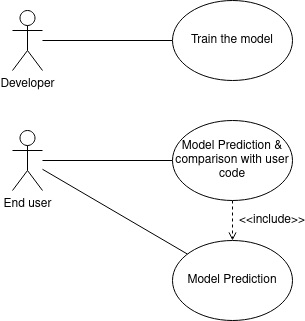
\includegraphics{use-case.drawio.png}    
    \caption{Діаграма прецедентів}
    \label{fig:use-case}
  \end{figure}

  \subsection{Внутрішнє проєктування}
  В додатку можна виділити наступні основні частини:
  \begin{itemize}[labelindent=\dimexpr\parindent*2\relax, leftmargin=*]
    \item інтерфейс користувача --- цей модуль буде перетворювати вхідні дані користувача на внутрішнє представлення та перевіряти коректність наданих даних. Також цей модуль відповідає за надання результату користувачу
    \item бекенд
      \begin{itemize}[labelindent=\dimexpr\parindent\relax, leftmargin=*]
        \item тренування моделі --- цей модуль буде додавати нові ключові слова до класів, знайдених у наданому тексті
        \item отримання припущення від моделі --- цей модуль буде надавати можливі класи до наданого тексту
        \item порівняння списків класів УДК --- цей модуль буде порівнювати два списки класів УДК, та надавати ступінь їх відповідності
      \end{itemize}
  \end{itemize}
  
  Також можна виділити такі типи даних (замість передавання рядка або числа між внутрішніми процедурами, зручніше передавати спеціалізовану структуру):
  \begin{itemize}[labelindent=\dimexpr\parindent*2\relax, leftmargin=*]
    \item наукова робота/текст,
    \item клас УДК.
  \end{itemize}

  \subsection{Проєктування архітектури системи}
  Програму розроблено ітераціями. На кожну з ітерацій виділено окрему секцію. Є два типи ітерацій:
  \begin{enumerate}[labelindent=\dimexpr\parindent*2\relax, leftmargin=*]
    \item Реалізація нового функціоналу,
    \item Вдосконалення старого функціоналу.
  \end{enumerate}
  Для простоти тестування було вирішено почати розробку з інтерфейсу користувача.
  З попередніх секцій знаємо що це буде інтерфейс командного рядка
  (CLI - Command Line Interface).

  Найпростішим варіантом
  є перевірка аргументів командного рядка у функції main,
  і після цього виклик із цими аргументами внутрішньої реалізації.

  UML-діаграма для такої моделі виглядає наступним чином
  (рис. \ref{fig:io_uml1}).
  Справжня реалізація буде мати складніший інтерфейс,
  але ця секція фокусуєтся на розробці користувацького інтерфейсу,
  тому на цьому єтапі реалізація представлена як дуже простий клас.

  \begin{figure}[H]
    \centering
    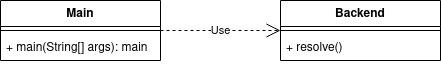
\includegraphics{io_uml1.drawio.png}    
    \caption{UML-діаграма 1}
    \label{fig:io_uml1}
  \end{figure}

  Алє таке рішення не є оптимальним ---
  заради простоти початкової реалізації
  втрачаєтся легкість подальшої заміні інтерфейсу.
  Тому доцільно виділити модуль який буде відповідати
  за взаємодію з користувачем.
  В нашому випадку це буде зчитування аргументів командного рядку,
  але за потреби він може бути замінений на графічний або веб-інтерфейс, тощо.
  Тепер діаграма виглядає так (рис. \ref{fig:io_uml2}).

  \begin{figure}[H]
    \centering
    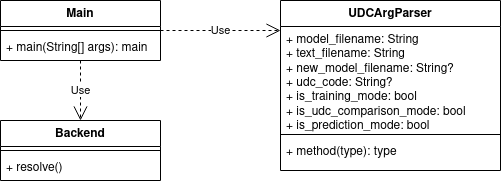
\includegraphics{io_uml2.drawio.png}    
    \caption{UML-діаграма 2}
    \label{fig:io_uml2}
  \end{figure}

  Тепер перед тим як викликати внутрішню реалізацію,
  main викликає клас UDCArgParser,
  який у свою чергу опрацьовує аргументи командного рядку.
  
  Хоча ця реалізація вирішує проблему відповідальності, вона додає декілька нових:
  \begin{itemize}[labelindent=\dimexpr\parindent*2\relax, leftmargin=*]
    \item по-перше UDCArgParser зчитує аргументи комадного рядка
    у конструкторі із глобальних змінних,
    це порушує принцип Dependency Inversion \cite{DI_wiki, SOLID_wiki};
    \item по-друге змінні is\_training\_mode, is\_udc\_comparison\_mode та \\ is\_prediction\_mode є взаємовиключними.
  \end{itemize}

  Для вирішення другої проблеми, потрібно скористатися поліморфізмом
  \cite{Polymorphism_wiki, Subtyping_wiki, Dynamic_dispatch_wiki}
  і замінити ці три змінні на одну,
  яка буде приймати значення одного з трьох підкласів.
  Іншими словами, треба заміни три взаємовиключні булеві змінні
  на одну змінну типу перечислення.
  З цими змінами UML-діаграма виглядає наступним чином (рис. \ref{fig:io_uml3}).

  \begin{figure}[H]
    \centering
    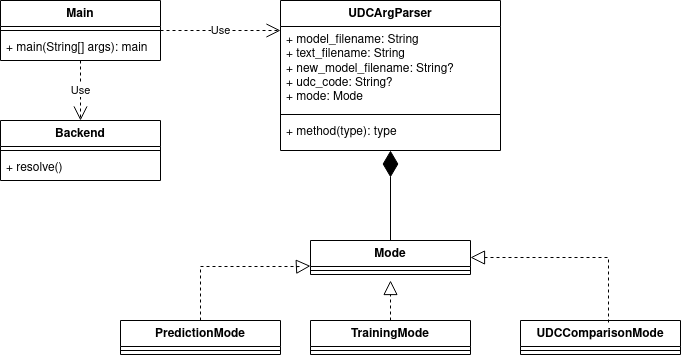
\includegraphics[width=\textwidth]{io_uml3.drawio.png}    
    \caption{UML-діаграма 3}
    \label{fig:io_uml3}
  \end{figure}
  
  Тепер клас Mode та його підкласи відповідають за представлення режиму,
  алє клас UDCArgParser має змінні new\_model\_filename та udc\_code,
  які в залежності від значення Mode завжди будуть NULL,
  тому доцільно перенести усі значення до підкласів Mode,
  перетворюючи тим самим це перечислення на алгебраічний тип данних
  \cite{ADT_wiki}.
  
  Доцільно помітити що алгебраічні типи даних відсутні в ООП та мові Python,
  тому вони будуть ємульовані з допомогою наслідування
  \cite{Code_complete_34_4, ADT_composition_over_inheritance}.
  
  Таким чином UDCArgParser дійсно буде мати тільки одну відповідальність ---
  перетворення аргументів командного рядка на об'єкт Mode.
  А Mode у свою чергу відповідає за представлення даних,
  які будуть надані внутрішній реалізації.
  Після цих змін UML-діаграма буде виглядати так (рис. \ref{fig:io_uml4}).

  \begin{figure}[H]
    \centering
    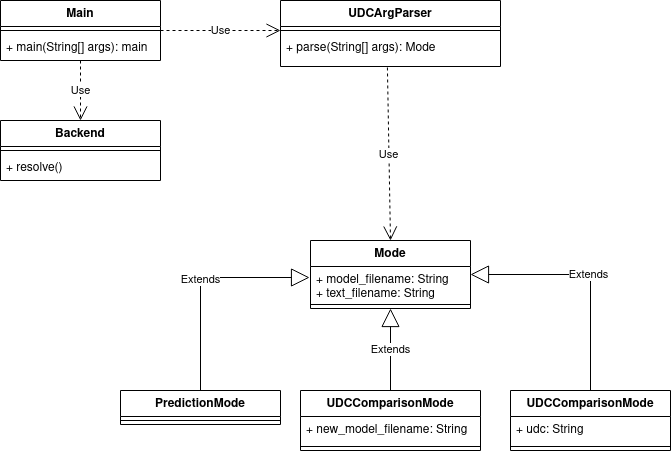
\includegraphics[width=\textwidth]{io_uml4.drawio.png}    
    \caption{UML-діаграма 4}
    \label{fig:io_uml4}
  \end{figure}
  
  Нова версія набагато краще попередніх, особливо першої.
  Втім все ще є недоліки:
  \begin{itemize}[labelindent=\dimexpr\parindent*2\relax, leftmargin=*]
    \item тип Mode містить поля model\_filename та text\_filename
    --- вони будуть передані в Backend
    (це не показано на діаграмах, тому теж є недоліком).
    Внутрішній реалізації потрібен вміст цих файлів,
    насправді внутрішня реалізація навіть не повинна знати що це вміст файлів,
    а не, наприклад, вміст текстового поля у графічному інтерфейсі, тощо.
    Тому доцільно:
      \begin{enumerate}[labelindent=\dimexpr\parindent\relax, leftmargin=*]
        \item Прибрати слово filename з обох полів,
        \item Виділити типи для цих значень ---
        таким чином ми зможемо робити майбутні зміни лише в одному місці
        \cite{Code_complete_5_3}
      \end{enumerate}
    \item Також присутня змінна new\_model\_filename в UDCComparisonMode ---
    вона так само не є важливою дла внутрішньої реалізації,
    а тільки для інтерфейсу користувача.
    Через те що для внутрішньої реалізації це буде одним з результатів
    (також можуть бути припущення щодо класів УДК та точності припущення,
    зробленного користувачем),
    це потрібно формалізувати в інтерфейсі класу Backend.
    \item Крім того, з попереднього пункту видно
    що потрібно формалізувати тип результату виконання внутрішньої реалізації.
    Втім, через те що маєтся чітка відовідність між підкласами Mode
    та типом (типами) результата внутрішньої реалізації доцільно розділити
    ці дії (режими роботи додатку) на окремі методи в класах Main та Backend.
  \end{itemize}

  У новій діаграмі (рис. \ref{fig:io_uml5})
  виділено типи UdcPredictorModel та UdcPredictorInput-Text,
  також явно показано залежність внутрішньої реалізації від типу Mode.

  UDCArgParser тепер має відповідальність
  за зчитування файлів за наданими іменами,
  але саме зчитування оброблюєтся внутрішньою бібліотекою мови Python,
  тому це не є порушення принципу єдиної відповідальності \cite{SRP_wiki}.
  Ця залежність не показана на діаграмі тому що вона подразумеваєтся/implied
  (я не знаю как перевести єто слово, googletranslate предлагает вообще не то)
  як атомарний функціонал мови, як і багато інших дещо простіших речей.

  Для вирішення інших проблем, описаних в попередній ітерації,
  краще розпочати з конкретизації внутрішньої реалізації.
  Через те що кожному з вхідних підтипів Mode буде відповідати новий формат
  результату, доцільно розділити метод resolve, на три різні.
  Крім того, ми можемо позбавитися залежності між
  внутрішньою реалізацією та типом Mode ---
  методи можуть приймати декілька параметрів,
  щодо результатів, функції в мові Python (та інших сучасних)
  можна повертати декілька значень
  \cite{python3_tuples_and_sequences}.

  \begin{sidewaysfigure}[htbp]
    \centering
    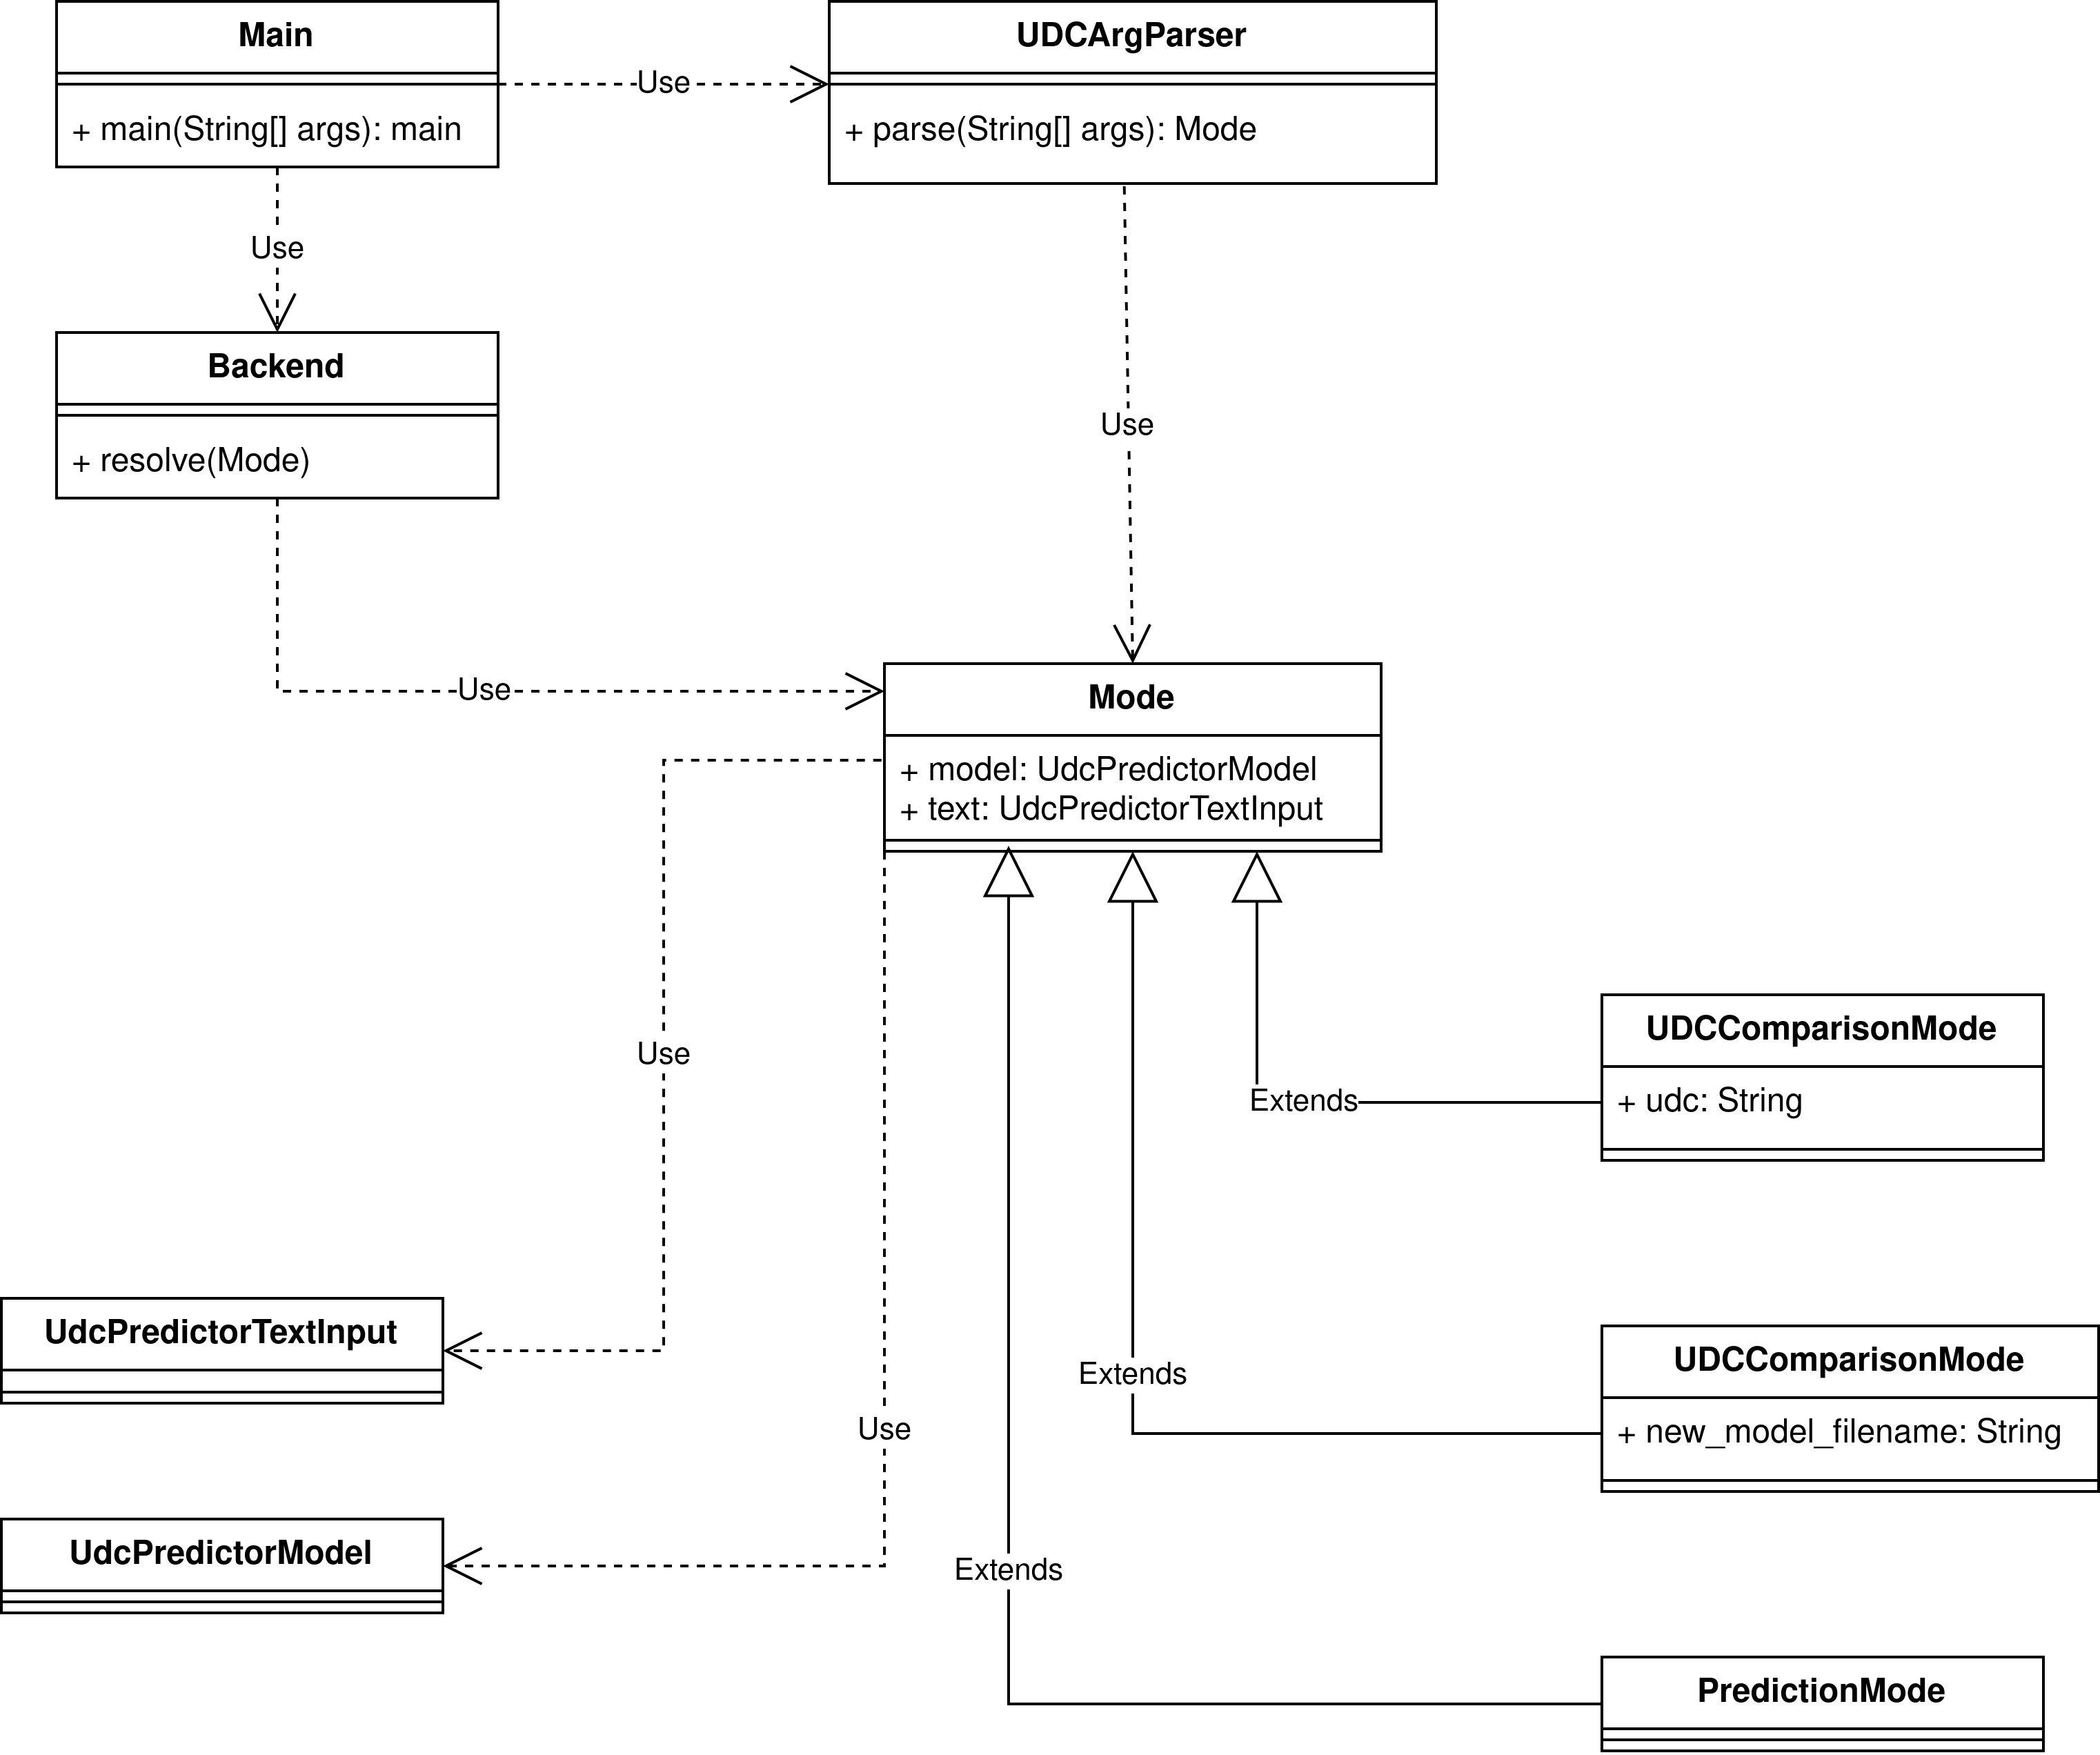
\includegraphics[height=0.6\textwidth]{io_uml5.drawio.png}    
    \caption{UML-діаграма 5}
    \label{fig:io_uml5}
  \end{sidewaysfigure}

  Через ці зміни, доцільно частково відмінити попередню зміну ---
  тип Mode буде мати імена файлів, а клас Main буде зчитувати та записувати їх.
  Це рішення є покращенням через те що тип
  UDCComparisonMode все ще має ім'я файлу,
  насправді його можна було б замінити на дескріптор файлу,
  алє тоді отримання ресурсу (файлу),
  та його звільнення (закриття) відбувалося б у різних методах та класах ---
  це порушує RAII \cite{wiki_raii}.
  Крім того, на даний момент клас Main не мав явної відповідальності
  (крім посередництва між іншими класами),
  тому ми можемо додати цю роботу до цього модуля.
  Також внутрішня реалізація буде напряму залежати
  від типів UdcPredictorTextInput та UdcPredictorModel.

  Нова версія (рис. \ref{fig:io_uml6}) вирішує вище описані проблеми
  наступним чином:
  \begin{itemize}[labelindent=\dimexpr\parindent*2\relax, leftmargin=*]
    \item внутрішня реалізація тепер має два методи ---
    припущення та тренування,
    вони напряму залежать від типів UdcPredictorModel та \\ UdcPredictorInputText.
    \item тип/клас/модуль UdcCode відподідає за представлення шифрів УДК
    та їх порівняння,
    модуль Main перетворює рядок отриманий від UdcArgParser на цей тип.
    \item усі взаємодії із файлами відбуваются у класі Main.
  \end{itemize}

  \begin{sidewaysfigure}[htbp]
    \centering
    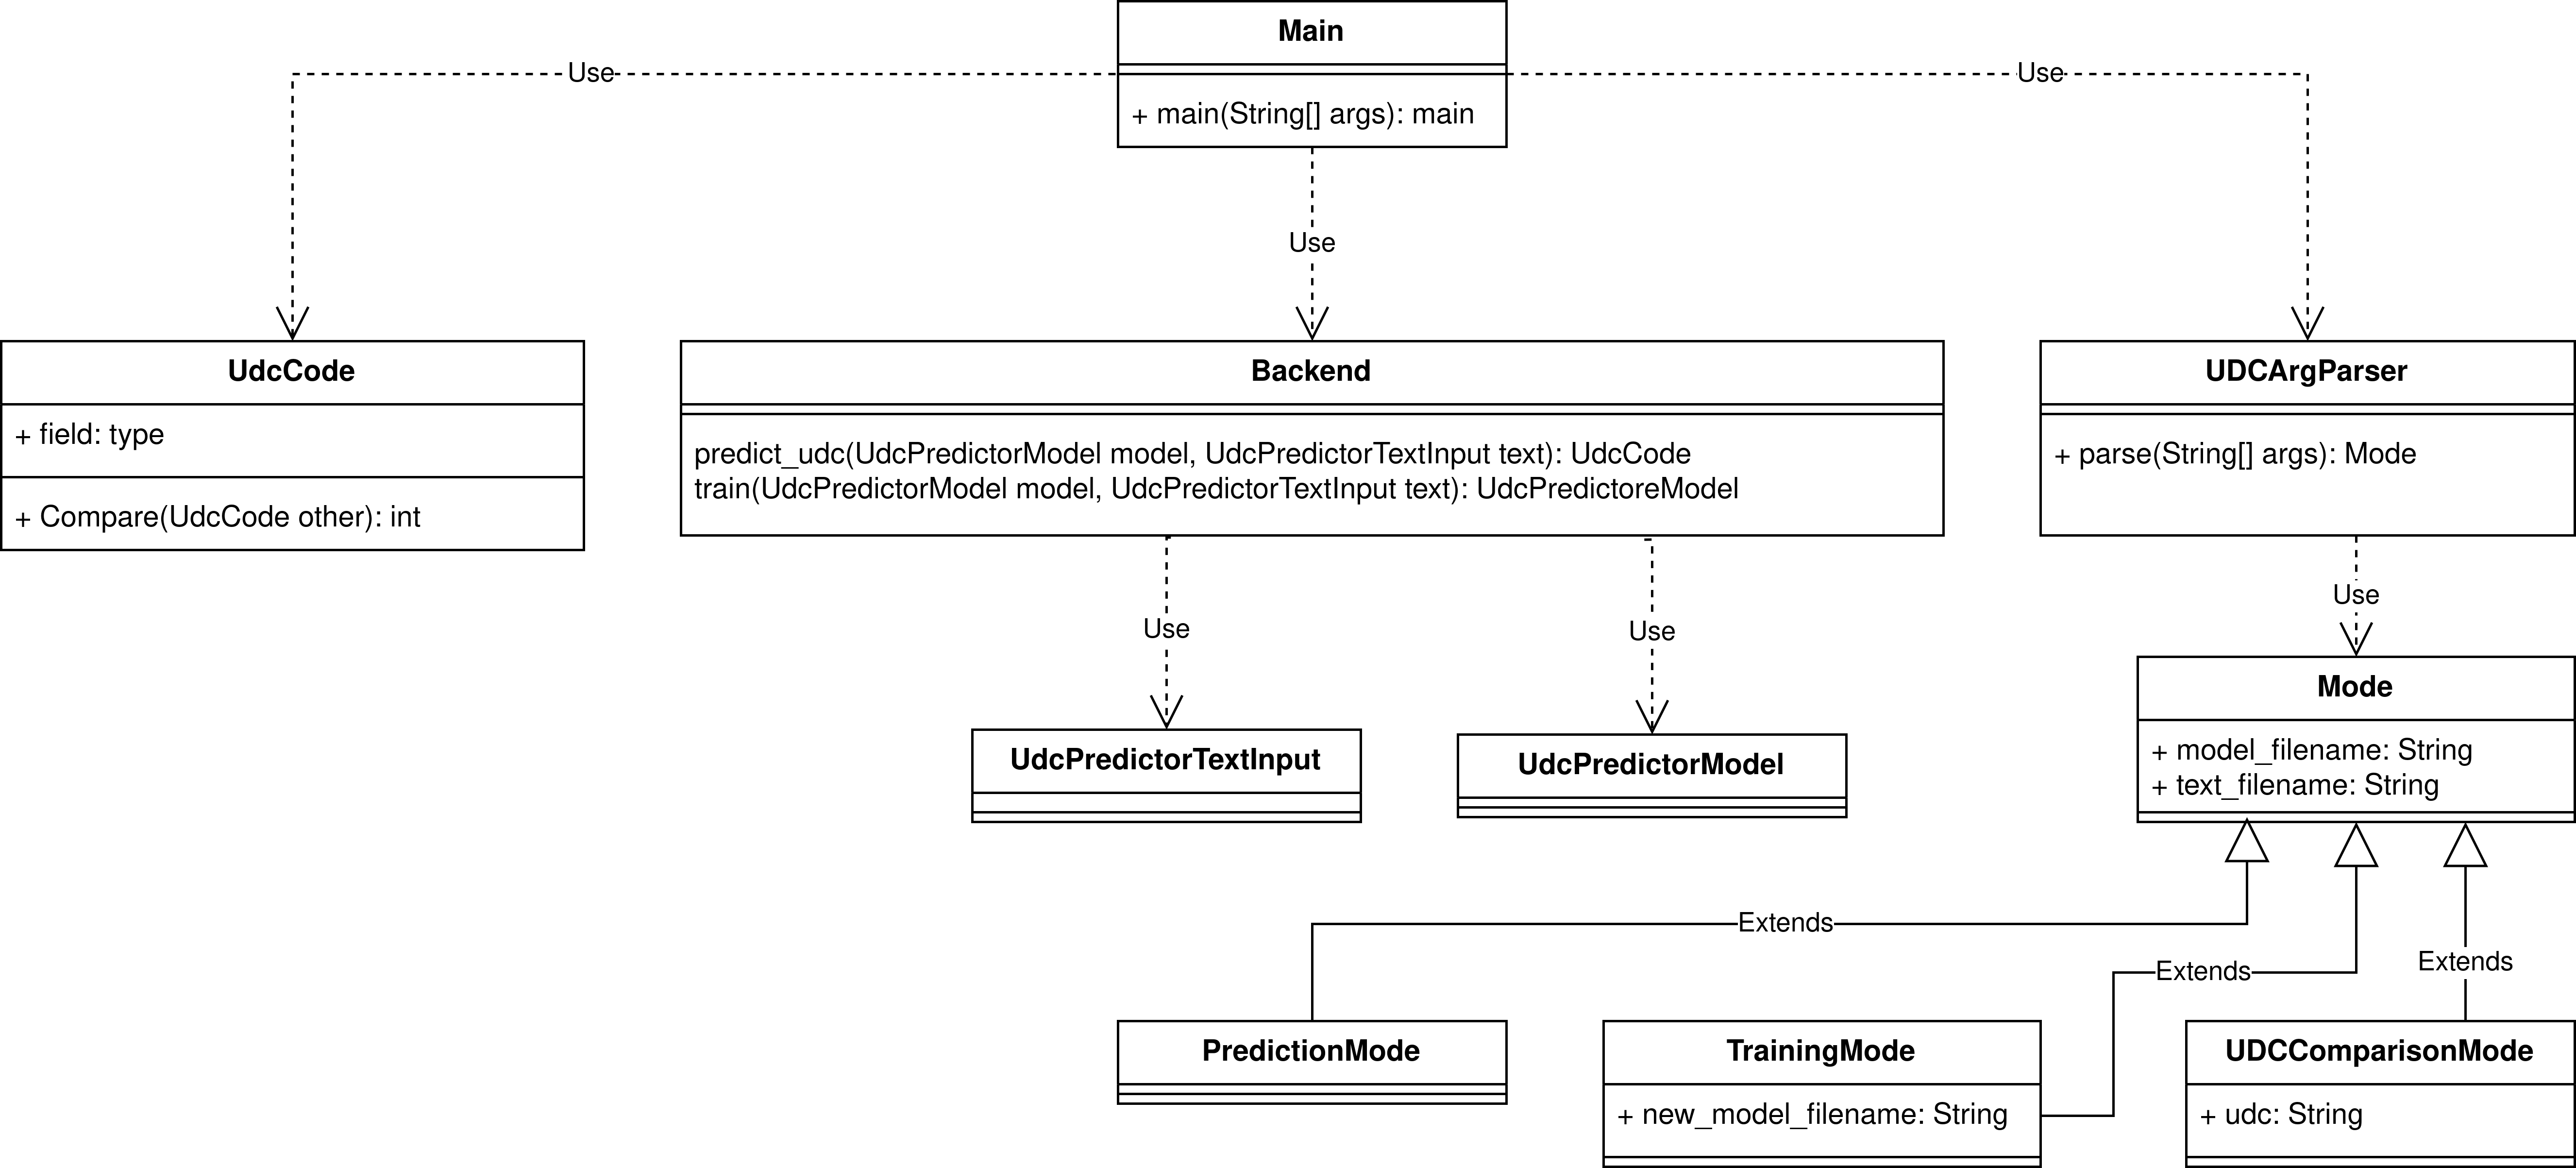
\includegraphics[height=0.45\textwidth]{io_uml6.drawio.png}    
    \caption{UML-діаграма 6}
    \label{fig:io_uml6}
  \end{sidewaysfigure}

  \newpage

  \subsection{Вибір засобів програмування}
  Для реалізації даного ПЗ було обрано мову Python,
  як найпопулярнішу в даному напрямі.
  Для вирішення задачі отримання ключових слів для заданого тексту
  потрібен такий функціонал:
  \begin{itemize}[labelindent=\dimexpr\parindent*2\relax, leftmargin=*]
    \item токенізація
    \item видалення стоп слів \cite{wiki_stop_word}
    \item розмічування частин мови \cite{wiki_pos_tagging}
    \item розпізнавання іменованих сутностей \cite{wiki_ner}
  \end{itemize}
  або готовий алгоритм виділення ключових слів.
  Знайдено такі бібліотеки зі схожим функціоналом:
  \begin{itemize}[labelindent=\dimexpr\parindent*2\relax, leftmargin=*]
    \item RAKE (Rapid Automatic Keyword Extraction) \cite{rake_nltk}
    \item YAKE (Yet Another Keyword Extractor) \cite{pypi_yake}
    \item spaCy \cite{spaCy}
    \item NLTK (Natural Language Toolkit) \cite{nltk}
    \item TextBlob \cite{TextBlob}
    \item Gensim \cite{gensim}
  \end{itemize}

  YAKE потребує тренування на конкретному наборі даних ---
  не підходить для цього випадку з тієї самої причини що й класифікація.

  TextBlob є високорівневою обгорткою над NLTK,
  тому їх доцільно розглядати разом.
  Це бібліотеки загального призначення,
  але їх можна відкинути з наступних причин:
  \begin{itemize}[labelindent=\dimexpr\parindent*2\relax, leftmargin=*]
    \item вони програють spaCy за швидкістю
    \item spaCy має кращі моделі
    \item spaCy має більш просунуті функції
  \end{itemize}

  Хоча spaCy не має готового алгоритму витягування ключових слів,
  його дуже легко реалізувати.

  Алгоритм, який використовує RAKE працює наступним чином ---
  текст розбивається на слова, потім перевіряється частота слів,
  та ступінь їх появи з іншими,
  слова сортуються за обома критеріями з попереднього кроку.

  spaCy не надає готово алгоритму виділення ключових слів,
  але дає можливість розбити текст на слова, розмічати їх як частини мови,
  розпізнати іменовані сутності.

  Алгоритм RAKE суто статистичний і має більшу похибку ---
  він може вважати за ключові слова такі,
  які не є вагомими та навпаки виключати важливі.

  Gensim не має деяких важливих алгоритмів
  для реалізації витягування ключових слів,
  а ті які є в цій бібліотеці були розроблені, в першу чергу,
  для інших цілей і не є оптимальними для нашої задачі.
  З цього виходить що spaCy є найкращим вибором:
  \begin{itemize}[labelindent=\dimexpr\parindent*2\relax, leftmargin=*]
    \item має весь потрібний функціонал;
    \item має моделі;
    \item швидше за інші бібліотеки.
  \end{itemize}

  \subsection{Перетворення ключових слів на класи УДК}
  В наведених у попередніх розділах відкритих каталогах УДК
  кількість ключових слів для кожного з підкласів дуже мала
  (близько 10 на кожен підклас), тому буде згенеровано свій каталог.
  Алгоритм створення наступний:
  \begin{enumerate}[labelindent=\dimexpr\parindent*2\relax, leftmargin=*]
    \item Беремо ключові слова з існуючої роботи (ті які надав автор),
    \item Витягуємо ключові слова з тексту з допомогою обраного алгоритму,
    \item Порівнюємо ключові слова з п.1 та п.2 та додаємо до каталогу ті,
    які входять до обох списків.
  \end{enumerate}

  Точність такого підходу буде напряму залежати від кількості розглянутих робіт
  та кількості отриманих ключових слів.
  Через обмежений час такі каталоги будуть створені не для усіх підкласів,
  та деякі класи будуть мати меншу вибірку.

  Для розуміння формату моделі,
  яка буде у подальшому використовуватися для припущень,
  доцільно деталізувати цей алгоритм.
  Так як модель буде змінюватися незалежно від коду --- це дані,
  які будуть зберігатися окремо від коду --- у файлі.
  Через це потрібно обрати формат серіалізації
  \cite{wiki_serialization,wiki_serialization_comparison}.

  \subsubsection{Вибір формату серіалізації}

  Для порівняння популярних форматів можна звернутися до статті
  «A Comparison Of Serialization Formats»
  \cite{mbedded_ninja_serialization_comparison} на веб-ресурсі mbedded.ninja
  \cite{mbedded_ninja}.

  Розглянемо критерії за якими ця стаття порівнює формати, та оберемо ті,
  які є важливими:

  \begin{itemize}[labelindent=\dimexpr\parindent*2\relax, leftmargin=*]
    \item Стислість --- цю характеристику можна вважати однією з складових
      читабельності,
      тому для простоти порівняння вона не буде включена у порівняльну таблицю.
    \item Читабельність --- хоча дані,
      які будуть серіалізуватися здебільшого орієнтовані на читання не людиною,
      а комп'ютером,
      іноді можуть виникати ситуації коли буде читабельність є важливою.
      Наприклад --- налагодження.
    \item Підтримка мов програмування --- ця характеристика є важливою
      для сумісності \cite{wiki_interop}
      з можливими розширеннями на інших мовах програмування.
    \item Структура даних --- ця характеристика має відносно низьку важливість.
      Вона має значення тільки у тих випадках, коли оцінка дуже низька,
      що свідчить про погану гнучкість
      і необхідність незручного перетворення деяких структур даних.
    \item Швидкість --- ця характеристика дуже залежна від реалізації
      тому не буде порівнюватися.
      Крім того, в цьому додатку швидкість не є критичною характеристикою,
      відповідно це стосуєтся і складових додатку.
    \item Стандартизація --- без цієї характеристики
      підтримка різних мов програмування має мало сенсу.
  \end{itemize}

  Важливі дані можна представити у вигляді таблиці
  (\ref{tab:serialization_comparison}).

  \begin{table}
    \centering
    \rotatebox{90}{
      \begin{minipage}{\textheight}
        \begin{tabular}{|c|c|c|c|c|}
          \hline
          Формат   & Підтримка мов програмування & Читабельність & Структура даних & Стандартизація \\
          CSV      & 9/10                        & 5/10          & 3/10            & 3/10 \\
          JSON     & 9/10                        & 5/10          & 6/10            & 9/10 \\
          Protobuf & 7/10                        & 1/10          & 8/10            & 9/10 \\
          TOML     & 6/10                        & 9/10          & 9/10            & 9/10 \\
          XML      & 9/10                        & 5/10          & 9/10            & 10/10 \\
          YAML     & 6/10                        & 7/10          & 10/10           & 8/10 \\
          \hline
        \end{tabular}
        \caption{Порівняння форматів серіалізації}
        \label{tab:serialization_comparison}
      \end{minipage}
    }
  \end{table}

  Одразу ж доцільно відкинути CSV \cite{wiki_csv}
  за низьку оцінку в структурі даних --- підтримуются тільки таблиці,
  та Protobuf \cite{wiki_protobuf} за дуже низьку оцінку в читабельності.

  Наступним кроком відкидаємо JSON \cite{wiki_json}
  та XML \cite{wiki_xml} через погану читабельність.

  Залишаєтся обрати з TOML \cite{wiki_toml} та YAML \cite{wiki_yaml}.
  Підтримка мов програмування у обох
  варіантів має однакову оцінку тому будемо обирати за іншими характеристиками.
  Найпростіше буде скласти інші оцінки та обрати варінт із більшою сумою,
  за таким порівняння виграє TOML (9+9+9=27) проти YAML (7+10+8=25).
  Можна також обрати той варіант який виграє по більшій кількості показників,
  тут також виграє TOML - два проти одного.

  Можна було б використати складніші способи порівняння,
  наприклад для кожної з обраних характеристик можна додавати множник
  важливості, і порівнювати суму значень з множниками.
  Алє на першому єтапі розробки для цього додатку це рішення не є практичним ---
  набагато краще було б отримати відгуки реальних користувачів,
  і вже на його основі можливо змінювати формат серіалізації,
  або додавати підтримку нового.

  Було обрано TOML (акронім "Tom's Obvious, Minimal Language").
  Крім вже оглянутих характеристик,
  можна додати що цей формат має синтаксис дещо схожий на Python,
  це можна вважати плюсом тому що дозволяє розробнику,
  та можливу користувачи витрачати меньше єнергії
  на перехід від коду до серіалізованих даних \cite{Code_complete_5_2}.
  Ця ситуація є схожою на JavaScript та JSON,
  тож якщо цей додаток був би написаний на JavaScript
  то JSON мав би додаткову перевагу.

  Крім того слід додати що вибір популярного
  та добре стандартизованого формату дозволяє мати більшу сумісність
  з іншими форматами завдяки конверторам з одного формату в інший
  \cite{github_json2toml,github_xmltodict,github_x2js}.
  
  \subsubsection{Формат моделі}

  \subsection{Висновки}

  \section{РОЗРОБКА ПРОГРАМИ}
  \subsection{Розробка інтерфейсу користувача}
  Для простоти виконання буде використано інтерфейс командного рядка (CLI). 
  Для цієї задачі в мові python є спеціалізований модуль argparse.

  З розробленої use-case діаграми можна сказати шо є два режими роботи
  (стільки  ж скільки й акторів).
  Через те що режими тільки два, доцільно використати прапор.
  Основним сценарієм є припущення,
  тому прапор буде використовуватися для тренування "\-\-training".
  
  Модель та текст присутні на вході кожного випадку,
  тому їх можна зробити позиційними аргументами.
  
  Список класів є тільки в одному випадку,
  тому це буде опціональним аргументом,
  який буде прийматися тільки якщо відсутній прапор "\-\-training",
  цей аргумент буде помічатись як "\-\-udc".
  Для припущення результат буде надаватися в stdout у наступному форматі:
  список класів та ступінь їх відповідності, якщо використано "\-\-udc".
  
  Маємо такі сценарії використання:
  \begin{enumerate}[labelindent=\dimexpr\parindent*2\relax, leftmargin=*]
    \item Тренування моделі
      \begin{mycode}[caption={Тренування моделі}, label={code:training_ex}]
        $ udc-classifier \
            model.model \
            scientific-work.txt \
            --training updated-model.model
      \end{mycode}
      \begin{itemize}
        \item udc-classifier --- назва виконуваного файлу
        \item model.model --- назва файлу існуючої моделі
        \item scientific-work.txt --- назва файлу з текстом наукової роботи
        \item updated-model.model --- назва файлу, до якого буде записано нову модель
      \end{itemize}
    
    \item Отримання припущення
      \begin{mycode}[caption={Отримання припущення}, label={code:result_prompt_ex}]
        $ udc-classifier model.model scientific-work.txt
      \end{mycode}
      \begin{mycode}[caption={Припущення (класи, які можуть підійти до наданого тексту)}
                    , label={code:result_ex}]
        539.120 94 084.3
      \end{mycode}
      \begin{itemize}
        \item udc-classifier --- назва виконуваного файлу
        \item model.model --- назва файлу існуючої моделі
        \item scientific-work.txt --- назва файлу з текстом наукової роботи
      \end{itemize}

    \item Отримання припущення та порівняння класів
      \begin{mycode}[caption={Отримання припущення та порівняння класів}, label={code:result_prompt_ex2}]
        $ udc-classifier \
            model.model \
            scientific-work.txt \
            --udc ‘913(574.22)"19"(084.3)’
      \end{mycode}
      \begin{mycode}[caption={Припущення}
                    , label={code:result_ex2}]
        539.120 94 084.3
        0.3
      \end{mycode}
      \begin{itemize}
        \item udc-classifier --- назва виконуваного файлу
        \item model.model --- назва файлу існуючої моделі
        \item scientific-work.txt --- назва файлу з текстом наукової роботи
        \item третій рядок прикладу ---
        класи, які можуть підійти до наданого тексту
        \item другий рядок --- вхідний шифр УДК
        \item четвертий рядок --- ступінь відповідності класів
        (від 0 до 1, де 0 --- відсутні співпадіння, 1 --- повне співпадіння)
      \end{itemize}
  \end{enumerate}


  \subsection{Висновки}

  \section{ТЕСТУВАННЯ ТА НАЛАГОДЖЕННЯ}
  \subsection{Поширенння додатку}
  Python це здебільшого інтерпретована мова програмування.
  Насправді некоретно казати що саме мова є інтерпретованою або компільованою,
  бо мова лише описує синтаксис та семантику,
  а код може бути і інтерпретованим і компільованим (напр. Dart \cite{dart_lang}),
  алє саме в мові Python офіційний інструмент для запуску програм ---
  інтерпретатор.
  
  Розроблюваний додаток орієнтований не тільки на просунутих користувачів,
  тому доцільно загорнути додаток в автономний пакет,
  щоб звільнити користувачів від встановлення інтерпретатора та бібліотек.

  Для вирішення цієї задачі можна розглянути декілька підходів:
  \begin{itemize}[labelindent=\dimexpr\parindent*2\relax, leftmargin=*]
    \item PyInstaller \cite{pyinstaller} ---
      один з головних претендентів на вирішення задачі.
      На перший погляд,
      ця python бібліотека повністю підходить під вказані вимоги ---
      вона збирає усі скрипти, усі модулі,
      усі бібліотеки та інтерпретатор в один комплект,
      який може бути запущеним кінцевим користувачем без додаткових дій.
      Втім, є деякі недоліки:
      \begin{itemize}
        \item це рішення не є кросплатформенним, тобто «зібрати» виконуваний файл для цільової платформи можна тільки на цій платформі
        \item деякі платформи зовсім не протестовані
      \end{itemize}
      Хоча це рішення є дуже гарним, доцільно розглянути й інші,
      перед тим як робити кінцевий вибір.
    
    \item Nuitka \cite{nuitka} --- python компілятор,
      так само не є кросплатформеним.
      Крім того, це рішення менш популярне ніж PyInstaller,
      та вимагає більшої кількості залежностей.
      Алє, це рішення може бути корисним, якщо додаток,
      зібраний з допомогою PyInstaller буде виконуватись дуже повільно.

    \item py2exe \cite{py2exe} --- цей інструмент орієнтований лише на одну
      операційну систему --- Windows,
      з цієї причини він є гіршим за інші запроновані рішення.
    
    \item Cython \cite{cython} --- самий популярний python компілятор.
    Хоча він також не має прямої можливості компілювати на інші платформи,
    він дозволяє компілювати в код на мові C,
    який у свою чергу можна компілювати на різні цільові платформи з однієї.
    Незважаючи на ці переваги, такий підхід не виграє по зручності PyInstaller,
    алє стоїть на приблизно тому самому рівні, завдяки перевагам над Nuitka.
    
    \item Frozen binaries \cite{github_cpython_freeze} ---
      функціонально те саме що й PyInstaller.
    
    \item Docker \cite{docker} ---
      ця система контейнеризації хоча й сама зручна та стандартизована
      з представлених, вимогає встановлення додаткового ПЗ ---
      через це, це решіння не має сенсу,
      бо ми намагаємося уникнути встановлення додаткового ПЗ
      та спростити встановлення розроблюваного додатку.
    
    \item Cloud-based deployment \cite{wiki_cloud_computing} ---
      найкраща сумістність з різними платформами,
      алє вимагає додаткових ресурсів, та постійного підключення до інтернету.
  \end{itemize}

  Для більш наглядного порівняння можна представити ці дані
  у вигляді такої таблиці:

  \begin{table}
    \centering
    \rotatebox{90}{
      \begin{minipage}{\textheight}
        \begin{tabular}{|c|c|c|c|c|c|c|}
          \hline
          Назва & Кросплатформеність & Тип & Windows & Linux & macOS & FreeBSD/NetBSD \\
          \hline
          PyInstaller & ні & Пакетувальник & 7/8/10/11 & + & >10.15 & +** \\
          Nuitka & ні & Компілятор & + & + & + & + \\
          py2exe & ні & Пакетувальник & + & - & - & - \\
          Cython & так* & Компілятор  & + & + & + & + \\
          Frozen binaries & ні & Пакетувальник  & + & + & + & + \\
          Docker & так & Kонтейнер  & + & + & + & + \\
          Cloud-based deployment & так & веб  & + & + & + & + \\
          \hline
        \end{tabular}

        \vspace{10pt}

        * - можна компілювати не у нативний код, а в код на мові С,
        а вже цей код можна крос-компілювати.

        ** - Неофіційна підтримка

        Nuitka потребує окремого встановлення компілятора gcc
      \end{minipage}
    }
  \end{table}

  \newpage
  З цієї таблиці можна побачити що усі варіанти мають
  підтримку усіх сучасних версій ОС Windows.
  Якщо відкинути py2exe,
  то будь який з варіантів підтримує усі сучасні/популярні ОС.
  Через це залишается обирати з варіантів,
  які дозволяють збирати виконувані файли з під однієї платформи на усі інші.
  Docker вже було виключено через
  те що він замінює одну залежніст від додаткового ПЗ на інше.
  Розгортання веб ресурсу також виключено через додаткові витрати.
  Залишаєтся лише Cython, який підтримує компіляцію на
  будь які цілові платформи з під однієї робочої.

  На практиці виявилося що крос-компіляція з Cython хоча й можлива,
  не є зручною. Головною причиною є погана сумісність компіляторів ---
  python на windows компілюєтся із допомогою компілятора MSVC,
  а крос-компіляція з linux на windows проводится із допомогою mingw.
  Цю проблему можна вирішити перекомпілювавши python із іншим компілятором,
  алє набагато легше буде використовувати цільові ОС для створення
  виконуваних файлів. Для цього доцільно використати PyInstaller.

  Для створення виконуваного файлу потрібно виконати такі кроки:
  \begin{enumerate}[labelindent=\dimexpr\parindent*2\relax, leftmargin=*]
    \item Перейти на цільову платформу.
    \item Встановити python --- для перевірки було використано версію 3.10,
      але скоріш за все підійдуть й інші.
    \item Встановити необхідні залежності:
      \begin{mycode}[caption={Встановлення залежностей}, label={code:install_deps}]
        > pip install spacy
        > python -m spacy download en_core_web_lg
        > pip install pyinstaller
      \end{mycode}
    \item Зібрати виконуваний файл за допомогою PyInstaller:
    \begin{mycode}[caption={Збірка виконуваного файлу}, label={code:install_deps}]
      > pyinstaller ^
          src\main.py ^
          -F ^
          --dist build ^
          --collect-all en_core_web_lg
    \end{mycode}
    Цей приклад використовувася на ОС Windows,
    але він буде працювати і на інших платформах. Єдина суттева зміна ---
    символ продовження строки (\string^), для віндовс це '\string^',
    для unix - '\string\'.
  \end{enumerate}

  В цілому, цей підхід вирішує проблему додаткових залежностей ---
  на виході маємо лише один виконуваний файл. Але можливі деякі покращення:
  \begin{itemize}[labelindent=\dimexpr\parindent*2\relax, leftmargin=*]
    \item Зараз мовна модель запаковуєтся в виконуваний файл.
      Для більшої універсальності можна зробити так,
      щоб модель знаходилась в окремій папці поряд із виконуваним файлом ---
      таким чином користувач за бажанням міг би замінити модель на іншу.
    \item Можна створити docker-контейнери з необхідними платформами
    \cite{docker_windows,docker_windows_base, docker_osx}
      та використовувати їх для збірки виконуваних файлів на
      різні цільові платформи з під однієї платформи розробки.
  \end{itemize}

  \subsection{Висновки}

  \unnumberedSection{ЗАГАЛЬНІ ВИСНОВКИ ТА РЕКОМЕНДАЦІЇ}
  \BgThispage

  \phantomsection
  \printbibliography[heading=bibintoc, title=СПИСОК ВИКОРИСТАНОЇ ЛІТЕРАТУРИ]

  \unnumberedSection{ДОДАТКИ}
  \BgThispage

\end{document}
